\section{Memorization with Low Computational Complexity}
\label{sec:reluach}

In this section, we introduce our ReLU network to memorize the input-output relationships $x_i \mapsto d_i,\,i=1,\ldots,n$. Our network will only yield $O(\log n)$ active neurons and weights per input. Application of Theorem \ref{th:synth} will then imply a conditional network that can achieve perfect recall with only $O(\log n)$ operations per input, as desired.

 Given a neural network $f$, and  an input $x$ to $f$, let $A(x;f)$ and $W(x;f)$ denote the number of active neurons and active weights, respectively. Our feedforward ReLU network construction is provided by the following theorem.
\begin{theorem}
\label{th:reluach}
Let $X = \{x_1,\ldots,x_n\}\subset\mathbb{R}^p$ be a dataset of input patterns such that for every $i,j\in\{1,\ldots,n\}$ with $i\neq j$, we have $x_i \neq x_j$. Let $\bar{x}_i = [\begin{smallmatrix} 1 \\ x_i \end{smallmatrix}]\in\mathbb{R}^{q}$, where $q=1+p$, be the augmented dataset patterns for biasing purposes. Let $d_1,\ldots,d_n\in\mathbb{R}^r$ be the corresponding desired outputs. Suppose every component of $d_i$ is non-negative for each $i\in\{1,\ldots,n\}$. Then, there is a neural network $f:\mathbb{R}^{q}\rightarrow\mathbb{R}^r$ such that for every $i\in\{1,\ldots,n\}$, we have $f(\bar{x}_i) = d_i$, 
\begin{align}
\label{eq:th1actneuronbound} 	A(\bar{x}_i;f) & \leq 2(q+1)\lceil \log_2 n \rceil + q+r \in O(r+q\log n), \\
%\end{align}
%and
%\begin{align}
\label{eq:th1actweightbound} 	W(\bar{x}_i;f)  & \leq 12q(q+1)\lceil \log_2 n \rceil + (r+2)q+r-2  \in O(rq+q^2\log n).
\end{align}



%\begin{align}
%\nonumber 
%A(\bar{x}_i;f) & \leq (q+r+2)\lceil \log_2 n \rceil + q+r-1 \\
%\label{eq:th1actneuronbound} & \in O((q+r)\log n).
%\end{align}
%Moreover, every neuron in network $f$ has at most $q$ incoming weights, resulting in $O(q(q+r)\log n)$ active weights per input according to (\ref{eq:th1actneuronbound}).


%the following statements hold.
%\begin{enumerate}[label={[\roman*]}]
%\item There is a neural network $f:\mathbb{R}^{q}\rightarrow\mathbb{R}^r$ and a constant $C_1\in\mathbb{R}$ such that $A(\bar{x}_i;f) \leq \log_2 n + C_1$ and $f(\bar{x}_i) = d_i,\,\forall i\in\{1,\ldots,n\}$.
%\item There is a neural network $f:\mathbb{R}^{q}\rightarrow\mathbb{R}^r$ and a constant $C_2\in\mathbb{R}$ such that $A(\bar{x}_i;f) \leq 2\log_2 n + C_2$ and $f(\bar{x}_i) = d_i,\,\forall i\in\{1,\ldots,n\}$. Each neuron in the network has in-degree at most $q=1+p$.
%\end{enumerate}
\end{theorem}
\begin{proof} (Sketch)
We provide an illustrative sketch of the proof. Suppose we wish to memorize the two-dimensional dataset given by Fig. \ref{fig:divideandconquera}. We can divide the datasets to two parts via a line, the resulting two parts to further two sub-parts, and so on, until reaching singletons, as shown in Fig. \ref{fig:divideandconquerb}. The overall network architecture that achieves the performance in the statement of the theorem is then shown in Fig. \ref{fig:nnforachievability}. The initial block $\mathbf{T}$ is a basic preprocessing translation. The ``switch'' $\mathbf{S}_{ij}$ corresponds to the line parameterized by weights $w_{ij}$ in Fig. \ref{fig:divideandconquerb}. The switch $\mathbf{S}_{ij}$ routes the zero vector to one output path and copy its input to the other output path, depending on the side of the $w_{ij}$-line its input vector resides. The switches are followed by ReLU neurons with weights $\gamma_i$. These neurons  map the corresponding input pattern on the active path to its desired output. Finally, the output of the $\gamma_i$-neurons are accumulated. As an example, the signals on the graph for input pattern $\bar{x}_6$ is provided, with $\bar{\bar{x}}_6 \triangleq \mathbf{T}(\bar{x}_6)$. In general, all input-output relationships are satisfied with $O(\log n)$ active neurons per dataset sample. We refer to the complete proof in Appendix \ref{sec:reluachthproofer} for the precise bounds.
\end{proof}

\begin{corollary}
	\label{toyotacorolla}
	Let $x_i,d_i,\,i=1,\ldots,n$ be a sequence of arbitrary input-output pairs as stated in Theorem \ref{th:reluach}. Then, there is a conditional network that, for every $i$, provides an output of $d_i$ whenever the input is $x_i$ by performing only $O(rq+q^2\log n)$ operations.
\end{corollary}
\begin{proof}
We apply the synthesis procedure in Theorem \ref{th:synth} to the network constructed in Theorem \ref{th:reluach}. An alternative more ``direct'' proof (that does not need Theorem \ref{th:synth}) is to implement the gating blocks $\mathbf{S}_{ij}$ in Fig. \ref{fig:divideandconquer} via if-else conditioning statements, resulting in a similar architecture.
\end{proof}



We recall that for ReLU networks without conditional computation, the best achievability result \cite{vardi2021optimal} requires $O(\sqrt{n\log n})$ neurons and weights for memorizing a dataset of size $n$. Since the construction in \cite{vardi2021optimal} is not optimized for conditional computation, it is easily observed that every input activates all $O(\sqrt{n\log n})$ neurons and weights of the network, resulting in $O(\sqrt{n \log n})$ active weights per input. In fact, the remarkable construction in \cite{vardi2021optimal} is a narrow network of a finite width of only $12$, but depth $O(\sqrt{n\log n})$. Even if every input activates only one neuron at each layer, one obtains $O(\sqrt{n\log n})$ active neurons or arithmetic operations per input. In contrast, we only need $O(\log n)$ active weights or operations (via Corollary \ref{toyotacorolla}) per input.


The fact that one cannot fundamentally achieve a sub-polynomial number of neurons without conditional computation is an easy consequence of the VC dimension theory. In our setting, the VC dimension corresponds to the cardinality of the largest dataset that can be memorized. Hence, upper bounds on the VC dimension translate to lower bounds on the memorization capacity. In this context, \cite[Theorem 8.6]{anthony1999neural} provides an $O(n_w^2)$ upper bound on the VC dimension for ReLU networks, where $n_w$ denotes the number of weights in the network. Since any upper bound on the VC dimension is also an upper bound on the cardinality of the largest possible dataset that can be memorized, we have $n \in O(n_w^2)$. It follows that $n_w \in \Omega(\sqrt{n})$ weights are the best possible for ReLU networks without conditional computation, meaning that the results of \cite{vardi2021optimal} are optimal up to logarithmic factors. Also, using the bound $n_w \leq n_e^2$, where $n_e$ is the number of neurons in the network (equality holds in the extreme scenario where every neuron is connected to every other neuron, including itself), we obtain the necessity of $\Omega(n^{1/4})$ neurons. 


\begin{figure}[h]\centerline{
     \begin{subfigure}[b]{0.45\textwidth}
\centerline{\scalebox{0.85}{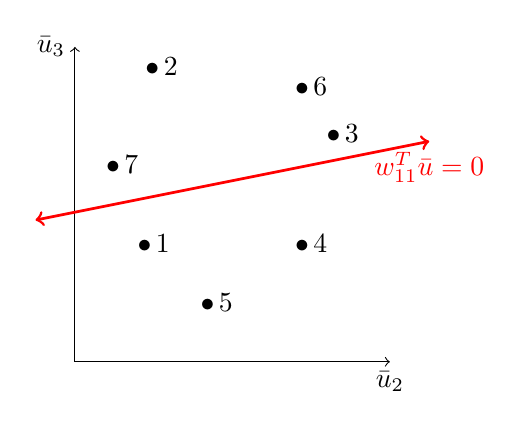
\begin{tikzpicture}

\draw[->] (0,0) -- (4,0) node[anchor=north] {$\bar{u}_2$};
\draw[->] (0,0) -- (0,4) node[anchor=east] {$\bar{u}_3$};
\draw (1,1.5) node {$\bullet\,1$}; %label
\draw (0.6,2.5) node {$\bullet\,7$}; %label
\draw (1.8,0.75) node {$\bullet\,5$}; %label
\draw (1.1,3.75) node {$\bullet\,2$}; %label
\draw (3.4,2.9) node {$\bullet\,3$}; %label
\draw (3,1.5) node {$\bullet\,4$}; %label
\draw (3,3.5) node {$\bullet\,6$}; %label
\draw[line width=1pt, red, <->] (-0.5,1.8) -- (4.5,2.8) node[anchor=north] {$w_{11}^T\bar{u} = 0$};
\end{tikzpicture}}}
\vspace{-5pt}
\caption{Dividing a set of point to two equal subsets.}
\label{fig:divideandconquera}
\end{subfigure}
     \begin{subfigure}[b]{0.45\textwidth}
\centerline{\scalebox{0.85}{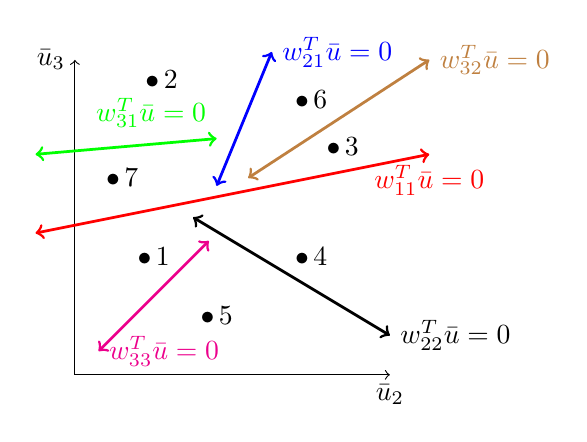
\begin{tikzpicture}

\draw[->] (0,0) -- (4,0) node[anchor=north] {$\bar{u}_2$};
\draw[->] (0,0) -- (0,4) node[anchor=east] {$\bar{u}_3$};
\draw (1,1.5) node {$\bullet\,1$}; %label
\draw (0.6,2.5) node {$\bullet\,7$}; %label
\draw (1.8,0.75) node {$\bullet\,5$}; %label
\draw (1.1,3.75) node {$\bullet\,2$}; %label
\draw (3.4,2.9) node {$\bullet\,3$}; %label
\draw (3,1.5) node {$\bullet\,4$}; %label
\draw (3,3.5) node {$\bullet\,6$}; %label
\draw[line width=1pt, red, <->] (-0.5,1.8) -- (4.5,2.8) node[anchor=north] {$w_{11}^T\bar{u} = 0$};
\draw[line width=1pt, blue, <->] (1.8,2.4) -- (2.5,4.1) node[anchor=west] {$w_{21}^T\bar{u} = 0$};
\draw[line width=1pt, brown, <->] (2.2,2.5) -- (4.5,4) node[anchor=west] {$w_{32}^T\bar{u} = 0$};
\draw[line width=1pt, black, <->] (1.5,2) -- (4,0.5) node[anchor=west] {$w_{22}^T\bar{u} = 0$};
\draw[line width=1pt, magenta, <->] (1.7,1.7) -- (0.3,0.3) node[anchor=west] {$w_{33}^T\bar{u} = 0$};
\draw[line width=1pt, green, <->] (-0.5,2.8) -- (1.8,3) node[anchor=south east] {$w_{31}^T\bar{u} = 0$};
\end{tikzpicture}}}
\vspace{-5pt}
\caption{Continued divisions until reaching singletons.}
\label{fig:divideandconquerb}
\end{subfigure}}
\vspace{-5pt}
\caption{The divide and conquer strategy.}
\label{fig:divideandconquer}
\end{figure}


%\begin{figure}
%\centerline{\begin{tikzpicture}[
%arrowstyle/.style={decoration={markings,mark=at position 1 with
%    {\arrow[scale=1.7,>=stealth]{>}}},postaction={decorate}},
%roundnode/.style={circle, draw=blue!60, fill=blue!5, very thick, minimum size=2mm},
%squarednode/.style={rectangle, draw=green!60, fill=yellow!5, very thick, minimum size=5mm},
%squarednode2/.style={rectangle, draw=magenta!60, fill=magenta!5, very thick, minimum size=5mm},
%squarednode3/.style={rectangle, draw=blue!60, fill=blue!5, very thick, minimum size=5mm},
%squarednode4/.style={rectangle, draw=red!60, fill=red!5, very thick, minimum size=5mm},]
%
%\node[inner sep=0pt, minimum size=3mm](n1x) at (-0.75,-0.5){$=[\begin{smallmatrix} 1 \\ x_6 \end{smallmatrix}]$};
%
%\node[inner sep=0pt, minimum size=3mm](n1) at (-1,0) {$u=\bar{x}_6$};
%\node[squarednode](t) at (0.5,0) {$\mathbf{T}$};
%\draw [arrowstyle](n1)--(t);
%\node[squarednode2](s11) at (2.5,0) {$\mathbf{S}_{11}$};
%\draw [arrowstyle](t)--node [below] {$\bar{u}=\bar{\bar{x}}_6$}(s11);
%\node[squarednode2](s21) at (4,1.8) {$\mathbf{S}_{21}$};
%\node[squarednode2](s22) at (4,-1.8) {$\mathbf{S}_{22}$};
%\draw [arrowstyle](s11)--node [below] {$\,\,\bar{\bar{x}}_6$}(s21);
%\draw [arrowstyle](s11)--node [below] {$0$}(s22);
%\node[squarednode2](s32) at (5.5,0.9) {$\mathbf{S}_{32}$};
%\node[squarednode2](s31) at (5.5,2.7) {$\mathbf{S}_{31}$};
%\node[squarednode2](s33) at (5.5,-2.7) {$\mathbf{S}_{33}$};
%
%\draw [arrowstyle](s21)--node [below] {$0$}(s31);
%\draw [arrowstyle](s21)--node [below] {$\!\!\bar{\bar{x}}_6$}(s32);
%\draw [arrowstyle](s22)--node [below] {$0$}(s33);
%
%\node[squarednode3](g2) at (7,3.15) {$\gamma_2^T$};
%\node[squarednode3](g2r) at (8,3.15) {$\relu$};
%
%\node[squarednode3](g7) at (7,2.25) {$\gamma_7^T$};
%\node[squarednode3](g7r) at (8,2.25) {$\relu$};
%
%\node[squarednode3](g6) at (7,1.35) {$\gamma_6^T$};
%\node[squarednode3](g6r) at (8,1.35) {$\relu$};
%
%\node[squarednode3](g3) at (7,0.45) {$\gamma_3^T$};
%\node[squarednode3](g3r) at (8,0.45) {$\relu$};
%
%\node[squarednode3](g5) at (7,-3.15) {$\gamma_5^T$};
%\node[squarednode3](g5r) at (8,-3.15) {$\relu$};
%
%\node[squarednode3](g1) at (7,-2.25) {$\gamma_1^T$};
%\node[squarednode3](g1r) at (8,-2.25) {$\relu$};
%
%\node[squarednode3](g4) at (7,-0.9) {$\gamma_4^T$};
%\node[squarednode3](g4r) at (8,-0.9) {$\relu$};
%
%\draw [arrowstyle](s31)--node [above] {$0$}(g2);
%\draw [arrowstyle](s31)--node [below] {$0$}(g7);
%\draw [arrowstyle](s32)--node [above] {$\bar{\bar{x}}_6$}(g6);
%\draw [arrowstyle](s32)--node [below] {$0$}(g3);
%\draw [arrowstyle](s22)--node [above] {$0$}(g4);
%\draw [arrowstyle](s33)--node [above] {$0$}(g1);
%\draw [arrowstyle](s33)--node [below] {$0$}(g5);
%
%\draw [arrowstyle](g1)--(g1r);
%\draw [arrowstyle](g2)--(g2r);
%\draw [arrowstyle](g3)--(g3r);
%\draw [arrowstyle](g4)--(g4r);
%\draw [arrowstyle](g5)--(g5r);
%\draw [arrowstyle](g6)--(g6r);
%\draw [arrowstyle](g7)--(g7r);
%
%
%\node[squarednode4](sumnode) at (10,0) {$\sum$};
%\draw [arrowstyle](g1r)--node [above] {$0$}(sumnode); 
%\draw [arrowstyle](g2r)--node [above] {$0$}(sumnode); 
%\draw [arrowstyle](g3r)--node [above] {$0$}(sumnode); 
%\draw [arrowstyle](g4r)--node [above] {$0$}(sumnode); 
%\draw [arrowstyle](g5r)--node [above] {$0$}(sumnode); 
%\draw [arrowstyle](g6r)--node [above] {$d_6$}(sumnode); 
%\draw [arrowstyle](g7r)--node [above] {$0$}(sumnode); 
%\node[squarednode4](sumnode2) at (11,0) {$\relu$};
%\draw [arrowstyle](sumnode)--(sumnode2); 
%\node[inner sep=0pt, minimum size=3mm](output) at (12,0) {$d_6$};
%\draw [arrowstyle](sumnode2)--(output); 
%
%
%\end{tikzpicture}}
%\caption{An example network architecture for the achievability result.}
%\label{fig:nnforachievability}
%\end{figure}
%
%\begin{figure}[h]
%\centerline{\scalebox{0.9}{\begin{tikzpicture}[
%arrowstyle/.style={decoration={markings,mark=at position 1 with
%    {\arrow[scale=1.7,>=stealth]{>}}},postaction={decorate}},
%roundnode/.style={circle, draw=blue!60, fill=blue!5, very thick, minimum size=2mm},
%squarednode/.style={rectangle, draw=green!60, fill=yellow!5, very thick, minimum size=5mm},
%squarednode2/.style={rectangle, draw=magenta!60, fill=magenta!5, very thick, minimum size=5mm},
%squarednode3/.style={rectangle, draw=blue!60, fill=blue!5, very thick, minimum size=5mm},
%squarednode4/.style={rectangle, draw=red!60, fill=red!5, very thick, minimum size=5mm},squarednode5/.style={rectangle, draw=orange!90, fill=orange!15, very thick, minimum size=5mm},]
%
%\node[inner sep=0pt, minimum size=3mm](n1x) at (-0.75,-0.5){$=[\begin{smallmatrix} 1 \\ x_6 \end{smallmatrix}]$};
%
%\node[inner sep=2pt, minimum size=3mm](n1) at (-1,0) {$u=\bar{x}_6$};
%\node[squarednode](t) at (0.5,0) {$\mathbf{T}$};
%\draw [arrowstyle](n1)--(t);
%\node[squarednode2](s11) at (2.5,0) {$\mathbf{S}_{11}$};
%\draw [arrowstyle](t)--node [below] {$\bar{u}=\bar{\bar{x}}_6$}(s11);
%\node[squarednode2](s21) at (4,1.8) {$\mathbf{S}_{21}$};
%\node[squarednode2](s22) at (4,-1.8) {$\mathbf{S}_{22}$};
%\draw [arrowstyle](s11)--node [below] {$\,\,\bar{\bar{x}}_6$}(s21);
%\draw [arrowstyle](s11)--node [below] {$0$}(s22);
%\node[squarednode2](s32) at (5.5,0.9) {$\mathbf{S}_{32}$};
%\node[squarednode2](s31) at (5.5,2.7) {$\mathbf{S}_{31}$};
%\node[squarednode2](s33) at (5.5,-2.7) {$\mathbf{S}_{33}$};
%
%\draw [arrowstyle](s21)--node [below] {$0$}(s31);
%\draw [arrowstyle](s21)--node [below] {$\!\!\bar{\bar{x}}_6$}(s32);
%\draw [arrowstyle](s22)--node [below] {$0$}(s33);
%
%\node[squarednode3](g2) at (7,3.15) {$\gamma_2$};
%\node[squarednode3](g7) at (7,2.25) {$\gamma_7$};
%\node[squarednode3](g6) at (7,1.35) {$\gamma_6$};
%\node[squarednode3](g3) at (7,0.45) {$\gamma_3$};
%\node[squarednode3](g5) at (7,-3.15) {$\gamma_5$};
%\node[squarednode3](g1) at (7,-2.25) {$\gamma_1$};
%\node[squarednode3](g4) at (7,-0.9) {$\gamma_4$};
%
%\draw [arrowstyle](s31)--node [above] {$0$}(g2);
%\draw [arrowstyle](s31)--node [below] {$0$}(g7);
%\draw [arrowstyle](s32)--node [above] {$\bar{\bar{x}}_6$}(g6);
%\draw [arrowstyle](s32)--node [below] {$0$}(g3);
%\draw [arrowstyle](s22)--node [above] {$0$}(g4);
%\draw [arrowstyle](s33)--node [above] {$0$}(g1);
%\draw [arrowstyle](s33)--node [below] {$0$}(g5);
%
%\node[squarednode5](s32sum) at (8.5,0.9) {$\sum$};
%\node[squarednode5](s31sum) at (8.5,2.7) {$\sum$};
%\node[squarednode5](s33sum) at (8.5,-2.7) {$\sum$};
%\node[squarednode5](s21sum) at (9.5,1.8) {$\sum$};
%\node[squarednode5](s22sum) at (9.5,-1.8) {$\sum$};
%\node[squarednode5](finalsum) at (10.5,0) {$\sum$};
%\node[inner sep=2pt, minimum size=4mm](output) at (11.5,0) {$d_6$};
%\draw [arrowstyle](finalsum)--(output); 
%
%\draw [arrowstyle](g2)--node [above] {$0$}(s31sum);
%\draw [arrowstyle](g7)--node [below] {$0$}(s31sum);
%\draw [arrowstyle](g6)--node [above] {$d_6$}(s32sum);
%\draw [arrowstyle](g3)--node [below] {$0$}(s32sum);
%\draw [arrowstyle](g4)--node [above] {$0$}(s22sum);
%\draw [arrowstyle](g1)--node [above] {$0$}(s33sum);
%\draw [arrowstyle](g5)--node [below] {$0$}(s33sum);
%
%\draw [arrowstyle](s33sum)--node [below] {$0$}(s22sum);
%\draw [arrowstyle](s32sum)--node [below] {$d_6$}(s21sum);
%\draw [arrowstyle](s31sum)--node [below] {$0$}(s21sum);
%\draw [arrowstyle](s21sum)--node [below] {$d_6$}(finalsum);
%\draw [arrowstyle](s22sum)--node [below] {$0$}(finalsum);
%
%
%\end{tikzpicture}}}
%\caption{An example network architecture for the achievability result. The block $\mathbf{T}$ represents the transformation in Step 1. Blocks $\mathbf{S}_{ij}$ are the routing switches. Blocks $\gamma_i$ represent ReLU neurons with weights $\gamma_i$, and $\sum$ blocks represent ReLU neurons with all-one weights.}
%\label{fig:nnforachievability}
%\end{figure}



\begin{figure}[h]
	\centerline{\scalebox{0.85}{\begin{tikzpicture}[
				arrowstyle/.style={decoration={markings,mark=at position 1 with
						{\arrow[scale=1.7,>=stealth]{>}}},postaction={decorate}},
				roundnode/.style={circle, draw=blue!60, fill=blue!5, very thick, minimum size=2mm},
				squarednode/.style={rectangle, draw=green!60, fill=yellow!5, very thick, minimum size=5mm},
				squarednode2/.style={rectangle, draw=magenta!60, fill=magenta!5, very thick, minimum size=5mm},
				squarednode3/.style={rectangle, draw=blue!60, fill=blue!5, very thick, minimum size=5mm},
				squarednode4/.style={rectangle, draw=red!60, fill=red!5, very thick, minimum size=5mm},squarednode5/.style={rectangle, draw=orange!90, fill=orange!15, very thick, minimum size=5mm},]
				
				\node[inner sep=0pt, minimum size=3mm](n1x) at (-0.75,-0.5){$=[\begin{smallmatrix} 1 \\ x_6 \end{smallmatrix}]$};
				
				\node[inner sep=2pt, minimum size=3mm](n1) at (-1,0) {$u=\bar{x}_6$};
				\node[squarednode](t) at (0.5,0) {$\mathbf{T}$};
				\draw [arrowstyle](n1)--(t);
				\node[squarednode2](s11) at (2.5,0) {$\mathbf{S}_{11}$};
				\draw [arrowstyle](t)--node [below] {$\bar{u}=\bar{\bar{x}}_6$}(s11);
				\node[squarednode2](s21) at (4,1.8) {$\mathbf{S}_{21}$};
				\node[squarednode2](s22) at (4,-1.8) {$\mathbf{S}_{22}$};
				\draw [arrowstyle](s11)--node [below] {$\,\,\bar{\bar{x}}_6$}(s21);
				\draw [arrowstyle](s11)--node [below] {$0$}(s22);
				\node[squarednode2](s32) at (5.5,0.9) {$\mathbf{S}_{32}$};
				\node[squarednode2](s31) at (5.5,2.7) {$\mathbf{S}_{31}$};
				\node[squarednode2](s33) at (5.5,-2.7) {$\mathbf{S}_{33}$};
				
				\draw [arrowstyle](s21)--node [below] {$0$}(s31);
				\draw [arrowstyle](s21)--node [below] {$\!\!\bar{\bar{x}}_6$}(s32);
				\draw [arrowstyle](s22)--node [below] {$0$}(s33);
				
				\node[squarednode3](g2) at (7,3.15) {$\gamma_2$};
				\node[squarednode3](g7) at (7,2.25) {$\gamma_7$};
				\node[squarednode3](g6) at (7,1.35) {$\gamma_6$};
				\node[squarednode3](g3) at (7,0.45) {$\gamma_3$};
				\node[squarednode3](g5) at (7,-3.15) {$\gamma_5$};
				\node[squarednode3](g1) at (7,-2.25) {$\gamma_1$};
				\node[squarednode3](g4) at (7,-0.9) {$\gamma_4$};
				
				\draw [arrowstyle](s31)--node [above] {$0$}(g2);
				\draw [arrowstyle](s31)--node [below] {$0$}(g7);
				\draw [arrowstyle](s32)--node [above] {$\bar{\bar{x}}_6$}(g6);
				\draw [arrowstyle](s32)--node [below] {$0$}(g3);
				\draw [arrowstyle](s22)--node [above] {$0$}(g4);
				\draw [arrowstyle](s33)--node [above] {$0$}(g1);
				\draw [arrowstyle](s33)--node [below] {$0$}(g5);
				
%				\node[squarednode5](s32sum) at (8.5,0.9) {$\sum$};
%				\node[squarednode5](s31sum) at (8.5,2.7) {$\sum$};
%				\node[squarednode5](s33sum) at (8.5,-2.7) {$\sum$};
%				\node[squarednode5](s21sum) at (9.5,1.8) {$\sum$};
%				\node[squarednode5](s22sum) at (9.5,-1.8) {$\sum$};
				\node[squarednode5](finalsum) at (9.5,0) {$\sum$};
				\node[inner sep=2pt, minimum size=4mm](output) at (10.5,0) {$d_6$};
				\draw [arrowstyle](finalsum)--(output); 
				
				\draw [arrowstyle](g2)--node [above] {$0$}(finalsum);
				\draw [arrowstyle](g7)--node [above] {$0$}(finalsum);
				\draw [arrowstyle](g6)--node [above] {$d_6$}(finalsum);
				\draw [arrowstyle](g3)--node [above] {$0$}(finalsum);
				\draw [arrowstyle](g4)--node [above] {$0$}(finalsum);
				\draw [arrowstyle](g1)--node [above] {$0$}(finalsum);
				\draw [arrowstyle](g5)--node [above] {$0$}(finalsum);
				
%				\draw [arrowstyle](s33sum)--node [below] {$0$}(s22sum);
%				\draw [arrowstyle](s32sum)--node [below] {$d_6$}(s21sum);
%				\draw [arrowstyle](s31sum)--node [below] {$0$}(s21sum);
%				\draw [arrowstyle](s21sum)--node [below] {$d_6$}(finalsum);
%				\draw [arrowstyle](s22sum)--node [below] {$0$}(finalsum);
%				
				
	\end{tikzpicture}}}
	\caption{An example network architecture for the achievability result. The block $\mathbf{T}$ represents the transformation in Step 1. Blocks $\mathbf{S}_{ij}$ are the routing switches. Blocks $\gamma_i$ represent ReLU neurons with weights $\gamma_i$, and the $\sum$ block represents a ReLU neuron with all-one weights.}
	\label{fig:nnforachievability}
\end{figure}

In contrast to the deep and narrow architecture that is optimal for unconditional computation, the network that achieves the performance in Theorem \ref{th:reluach} is considerably wider but much shallower. In fact, the proof in Appendix \ref{sec:reluachthproofer} reveals that our network has width $O(n)$, with $O(n)$ nodes, and depth $O(\log n)$. These numbers are a consequence of the classical binary decision tree that we utilize in our network construction. Thanks to conditional computation, although the network has $O(n)$ nodes, every dataset pattern activates only $O(\log n)$ neurons instead of $O(\sqrt{n})$ neurons without conditional computation. Note that the function $\log n$ grows much slower than $\sqrt{n}$ so that the number of neurons activated by the conditional computation is asymptotically negligible relative to an unconditional network. Moreover, every neuron in the conditional computation network has a bounded number of $q$ weights. The two facts translate to  big savings in terms of the cost of computation, thanks to Theorem \ref{th:synth}. An interesting open problem that we shall leave as future work is whether one can achieve the same performance with a much smaller network size, e.g. with $O(\sqrt{n})$ neurons, which is known to be optimal. This will also help reduce the size of the network synthesized by Theorem \ref{th:synth}.



It should be mentioned that the bounds (\ref{eq:th1actneuronbound}) and (\ref{eq:th1actweightbound}) on the number of active neurons and weights as stated in Theorem \ref{th:reluach} holds only for input patterns that belong to the dataset. For such patterns, only one path from the input to the output of the neural network is activated. The global behavior of the neural network for arbitrary inputs is more complex. A careful analysis of the construction in Appendix \ref{sec:reluachthproofer}  reveals that near the decision boundaries (the lines in Fig. \ref{fig:divideandconquerb}), multiple paths of the network are activated, This will result in more active neurons and weights than what is suggested by the upper bounds in (\ref{eq:th1actneuronbound}) and (\ref{eq:th1actweightbound}), respectively. However, the measure of such pathological inputs can be made arbitrarily small by tuning the switches appropriately.

\label{sec:reluachthdiscuss}